%%%%%%%%%%%%%%%%%%%%%%%%%%%%%%%%%%%%%%%%%
% In The Name of God
%
%
% Parham Alvani Resume/CV
% parham.alvani@gmail.com
% https://github.com/1995parham
%
%%%%%%%%%%%%%%%%%%%%%%%%%%%%%%%%%%%%%%%%%

%%%%%%%%%%%%%%%%%%%%%%%%%%%%%%%%%%%%%%%%%
% Friggeri Resume/CV
% XeLaTeX Template
% Version 1.2 (3/5/15)
%
% This template has been downloaded from:
% http://www.LaTeXTemplates.com
%
% Original author:
% Adrien Friggeri (adrien@friggeri.net)
% https://github.com/afriggeri/CV
%
% License:
% CC BY-NC-SA 3.0 (http://creativecommons.org/licenses/by-nc-sa/3.0/)
%
% Important notes:
% This template needs to be compiled with XeLaTeX and the bibliography, if used,
% needs to be compiled with biber rather than bibtex.
%
%%%%%%%%%%%%%%%%%%%%%%%%%%%%%%%%%%%%%%%%%

\documentclass[]{friggeri-cv} % Add 'print' as an option into the square bracket to remove colors from this template for printing

\usepackage{parham-cv}

\begin{document}

% Your name and current job title/field
\header{Parham}{Alvani}{MSc. Student of Computer Networks}

%----------------------------------------------------------------------------------------
%	SIDEBAR SECTION
%----------------------------------------------------------------------------------------

\begin{aside} % In the aside, each new line forces a line break
	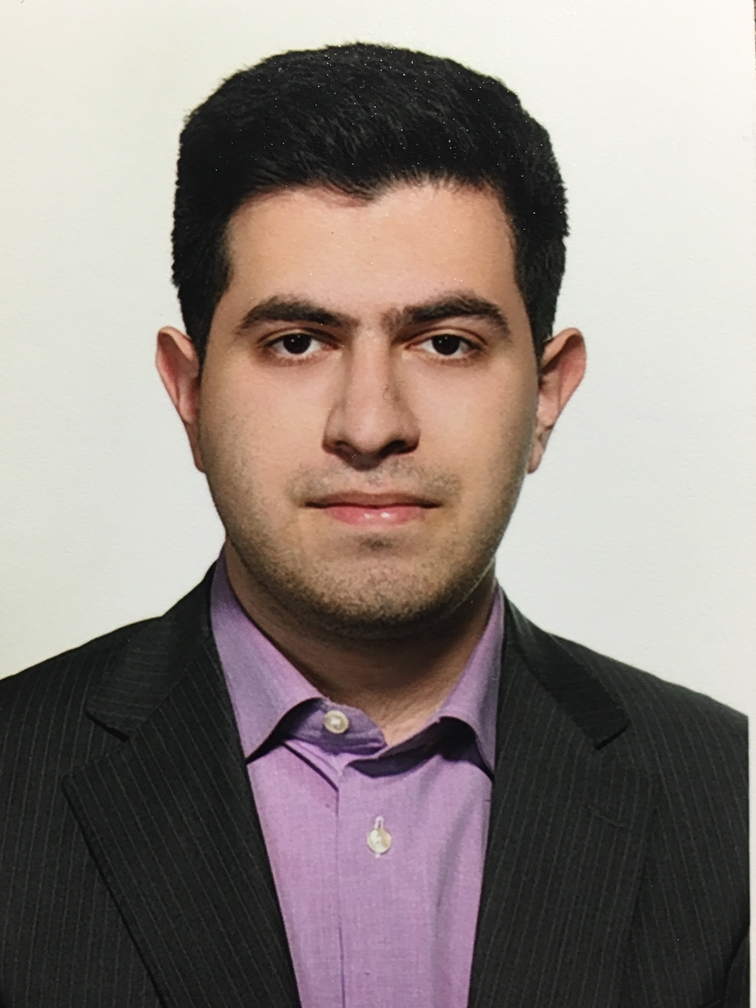
\includegraphics[width=3cm, height=4cm]{../parham_alvani_pers.jpg}
	\section{\textcolor{TextYellow}{c}ontact}
	Amirkabir University of Technology,
	Hafez Ave,
	Tehran, Iran
	---
	\href{mailto:parham.alvani@gmail.com}{parham.alvani@gmail.com}
	\href{mailto:parham.alvani@aut.ac.ir}{parham.alvani@aut.ac.ir}
	\href{https://1995parham.github.io/}{1995parham.github.io}
	\section{\textcolor{TextOrange}{l}anguages}
	Persian (Farsi):
	Native proficiency
	English:
	Limited working proficiency
	\section{\textcolor{TextGreen}{p}rogramming}
	{\color{red} $\varheartsuit$} C, Go, Python3, Node
	PHP
	AMD64 Assembly,
	AVR Assembly,
	Java SE, Java EE
	CSS3 \& HTML5
	JS
	\section{\textcolor{DarkBlue}{p}rojects}
	\href{https://github.com/1995parham}{\textcolor{TextGreen}{Github}}
	\section{\textcolor{Ocean}{last}-update}
	\today
\end{aside}

%----------------------------------------------------------------------------------------
%	INTERESTS SECTION
%----------------------------------------------------------------------------------------

\section{interests}
\textbf{professional:}
\begin{itemize}
	\item Internet of Things (IoT)
	\item Software Defined Networking (SDN)
	\item Network Function Virtualization (NFV)
	\item Kernel Hacking
	\item Mathematical Optimization
\end{itemize}
\textbf{personal:}
\begin{itemize}	
	\item Chess
\end{itemize}


%----------------------------------------------------------------------------------------
%	EDUCATION SECTION
%----------------------------------------------------------------------------------------

\section{education}

\begin{entrylist}

	%------------------------------------------------

	\entry{2017--2019}
	{Master \normalfont{of Computer Networks}}
	{Amirkabir University of Technology}
	{GPA:\@ 18.77/20}

	%------------------------------------------------

	\entry{2013--2017}
	{Bachelor \normalfont{of Computer Software Engineering}}
	{Amirkabir University of Technology}
	{GPA:\@ 18.94/20}

	%------------------------------------------------

	\entry{2009--2013}
	{High School, \normalfont{Diploma of Math \& Physics}}
	{Energy Atomic High School}
	{GPA:\@ 19.45/20}

	%------------------------------------------------


\end{entrylist}
\pagebreak

%----------------------------------------------------------------------------------------
%	HONORS and AWARDS SECTION
%----------------------------------------------------------------------------------------

\section{honors \& awards}

\begin{entrylist}
	
	\entry{Summer 2017}
	{\normalfont{Qualified to} \textcolor{UniBlue}{Direct Admission} \normalfont{to graduate school (M.Sc.) of Computer Engi- neering and IT Department, AUT}}
	{}
	{}

	%------------------------------------------------

	\entry{Summer 2016}
	{\normalfont{Achieved} \textcolor{TextOrange}{10th} \normalfont{Place in Final National Scientific Olympiad in Computer Engineering}}
	{}
	{}

	%------------------------------------------------

	\entry{Spring 2016}
	{\normalfont{Achieved} \textcolor{TextOrange}{4th} \normalfont{Place in Semi-Final National Scientific Olympiad in Computer Engineering}}
	{}
	{}
	
	%------------------------------------------------

	\entry{Spring 2016}
	{\normalfont{Achieved} \textcolor{TextYellow}{2nd} \normalfont{Place in 3rd National Digital Design Contest of Iran ASIC League as a Member of \emph{Polytechnic} team}}
	{}
	{}

	%------------------------------------------------

	\entry{Spring 2016}
	{\normalfont{Achieved} \textcolor{TextYellow}{3rd} \normalfont{Place in 3rd National Digital Design Contest of Iran CoDesign League as a Member of \emph{Polytechnic} team}}
	{}
	{}

	%------------------------------------------------

	\entry{2015}
	{\normalfont{Eligible to choose} \textcolor{TextGreen}{second major} \normalfont{due to outstanding performance}}
	{}
	{}

	%------------------------------------------------

	\entry{Spring 2015}
	{\normalfont{Awarded as an Outstanding Student by the head of Computer Engineering and Information Technology department, AmirKabir University of Technology}}
	{}
	{}

	%------------------------------------------------

	\entry{Spring 2015}
	{\normalfont{Achieved} \textcolor{TextYellow}{3rd} \normalfont{Place in 2nd National Digital Design Contest of Iran CoDesign League as a Member of \emph{Polytechnic} team}}
	{}
	{}

	%------------------------------------------------

	\entry{Fall 2014}
	{\normalfont{Achieved} \textcolor{UniBlue}{3rd} \normalfont{Place in 14th Amirkabir ACM International Collegiate Programming Contest (ICPC) as a Member of \emph{703} team}}
	{}
	{}

	%------------------------------------------------

	\entry{Fall 2014}
	{\normalfont{Participated in 39th Asia Regional ACM International Collegiate Programming Contest (ICPC) in Sharif University of Technology as a Member of \emph{703} team}}
	{}
	{}

	%------------------------------------------------

	\entry{2013}
	{\normalfont{Ranked in $0.2\%$ among more than $251,956$ participators in Nation-wide University Entrance Exam among all Iranian Students of Math. \& Physics}}
	{}
	{}

	%------------------------------------------------

	\entry{2012}
	{\textcolor{TextOrange}{Semi-finalist} \normalfont{at National Mathematics and Computer Olympiads}}
	{}
	{}

	%------------------------------------------------

	\entry{2011}
	{\textcolor{TextOrange}{Semi-finalist} \normalfont{at National Mathematics and Computer Olympiads}}
	{}
	{}

	%------------------------------------------------

	\entry{2010}
	{\textcolor{TextOrange}{Semi-finalist} \normalfont{at National Mathematics and Computer Olympiads}}
	{}
	{}

	%------------------------------------------------

	\entry{2010}
	{\normalfont{Achieved} \textcolor{Ocean}{Merit Award} \normalfont{in the International Mathematics Competition (IMC) Icheon, South Korea}}
	{}
	{}

	%------------------------------------------------

	\entry{2006--2009}
	{\normalfont{Member of National Organization for Development of Exceptional Talents \href{https://en.wikipedia.org/wiki/National_Organization_for_Development_of_Exceptional_Talents}{(NODET)}}}
	{}
	{}


\end{entrylist}
\pagebreak

%----------------------------------------------------------------------------------------
%       RESEARCH EXPERIENCE
%----------------------------------------------------------------------------------------

\section{research experience}

\begin{entrylist}
	\entry{M.Sc. Project}
	{SFC Requests Admission Control by Considering VNFMs}
	{Under supervision of Prof.Bakhshi}
	{Maximize profit optimization problem for accepting SFCs and provides VNFMs for them}
	
	\entry{B.Sc. Project}
	{General purpose IoT platform, design for scalability}
	{Under supervision of Prof.Sabaei}
	{Research and develop Distributed, Docker based IoT Platform named \href{https://github.com/bambil/bamboo}{Bamboo}}
	
	\entry{2015--2016}
	{Department-wide platform for IoT and building management systems}
	{Under supervision of Prof.Bakhshi, \href{https://aolab.github.io/}{AoLab}}
	{Research on different operating systems, frameworks and protocol stacks in IoT}
	
	\entry{2016--2017}
	{Middleware platform for IoT based on agent based approch}
	{Under supervision of Prof.Bakhshi, \href{https://aolab.github.io/}{AoLab}}
	{Research and develop \href{https://I1820.github.io}{I1820}}

	\entry{Spring 2016}
	{Resource Provisioning in Sotfware Defined Networking}
	{P.\ Alvani}
	{This research was done for Research Method and Technical Writings course}

\end{entrylist}

%----------------------------------------------------------------------------------------
%       WORK EXPERIENCE
%----------------------------------------------------------------------------------------

\section{work experience}

\begin{entrylist}

	\entry{Summer 2016}
	{IoT hardware and sotfware developer}
	{Iranian Telecommunication Reseach Center ITRC, Tehran, Iran}
	{Summer internship in the country's leading research center of telecommunication network systems}

	\entry{2017--2018}
	{LoRa enabled platform for smart agriculture}
        {IoT Working Group of Amirkabir University of Technology, Tehran, Iran}
	{System Architect and Developer}

	
\end{entrylist}

%----------------------------------------------------------------------------------------
%       EXTRA-CURRICULAR ACTIVITY
%----------------------------------------------------------------------------------------

\section{extra-curricular activity}

\begin{entrylist}

	\entry{Spring 2016}
	{Scientific Director}
	{}
	{Linux Festival}
	\entry{Fall 2016}
	{Techinal Team Member}
	{}
	{ACM ICPC}
	\entry{Spring 2017}
	{Scientific Director}
	{}
	{Linux Festival}
	\entry{Fall 2017}
	{Head of Technical Team}
	{}
	{ACM ICPC}
	\entry{Fall 2018}
	{Head of Technical Team}
	{}
	{ACM ICPC}
	
\end{entrylist}

\pagebreak

%----------------------------------------------------------------------------------------
%       SKILLS and EXPERTISE
%----------------------------------------------------------------------------------------

\section{skills \& expertise}

\begin{entrylist}

	\entry{\textcolor{TextGreen}{$\bullet$}}
	{Functional Programming Languages}
	{}
	{SML, Lisp, Haskell}

	%------------------------------------------------

	\entry{\textcolor{TextOrange}{$\bullet$}}
	{Hardware Definition Languages}
	{}
	{Verilog HDL, VHDL, Spice}

	%------------------------------------------------

	\entry{\textcolor{DarkBlue}{$\bullet$}}
	{Networking Tools and Protocols}
	{}
	{ONOS Platform, FloodLight, Ryu, Mininet, GNS3, Wireshark, Cisco Packet Tracer, OpenFlow1.3, OpenFlow1.5}

	%------------------------------------------------

	\entry{\textcolor{Ocean}{$\bullet$}}
	{Typesetting}
	{}
	{\LaTeX, Microsoft Word, LibreOffice, Pages, Vim}

	%------------------------------------------------

	\entry{\textcolor{LightGray}{$\bullet$}}
	{Hardware Simulators}
	{}
	{Xilinx Vivado Design Suite, P-Spice, H-Spice, Proteus, Quartus II}

	%------------------------------------------------

	\entry{\textcolor{TextYellow}{$\bullet$}}
	{DB Management Systems}
	{}
	{MySQL, PostgreSQL, MongoDB, Microsoft SQL Server}

	%------------------------------------------------

	\entry{\textcolor{TextRed}{$\bullet$}}
	{Operating Systems}
	{}
	{Ubuntu Desktop, Ubuntu Server, CentOS, OS X, Windows, Windows Server 2012, VMware vSphere 6.5}

	%------------------------------------------------

	\entry{\textcolor{TextPink}{$\bullet$}}
	{Other}
	{}
	{Netbeans, IntelliJ, Eclipse, Octave, Matlab}

	%------------------------------------------------

	\entry{\textcolor{UniBlue}{$\bullet$}}
	{Frameworks}
	{}
	{
		\textbf{Virtualization Frameworks}
		\begin{itemize}
			\item Docker
			\item Docker Compose
			\item OpenVSwitch
		\end{itemize}
		\textbf{C Frameworks}
		\begin{itemize}
			\item CGI Programming
			\item BSD Socket Programming
			\item UNIX System Programming
			\item GTK
			\item Gnome
		\end{itemize}
	
		\textbf{Java Frameworks}
		\begin{itemize}
			\item Maven
			\item Log4j
			\item JPA (Java Persistence API)
			\item Hibernate
			\item JSP
			\item JSF
		\end{itemize}
	}

	%------------------------------------------------


\end{entrylist}
\pagebreak

%----------------------------------------------------------------------------------------
%       TEACHING EXPERIENCES
%----------------------------------------------------------------------------------------

\section{teaching experiences}

\begin{entrylist}

	\entry{Fall 2014, 2015, 2016, 2017, 2018}
	{Principles of Computer and Programming}
	{Teaching Assistant}
	{Amirkabir University of technology, Under Supervision of Prof.\ Bakhshi.}

	%------------------------------------------------

	\entry{Spring 2015, 2016, 2018}
	{Advance Programming}
	{Teaching Assistant}
	{Amirkabir University of technology, Under Supervision of Prof.\ Noorhosseini.}

	%------------------------------------------------

	\entry{Spring 2015}
	{Discrete Mathematics}
	{Teaching Assistant}
	{Amirkabir University of technology, Under Supervision of Prof.\ Fallah.}

	%------------------------------------------------

	\entry{Spring 2015}
	{Introduction to Python Programming}
	{Instructor}
	{7th Amirkabir Linux Festival, Python Workshop}

	%------------------------------------------------

	\entry{Spring 2016, 2017}
	{Principles of Database Design}
	{Teaching Assistant}
	{Amirkabir University of technology, Under Supervision of Prof.\ Momtazi.}

	%------------------------------------------------

	\entry{Spring 2016, 2018, Fall 2018}
	{Microprocessor I}
	{Teaching Assistant}
	{Amirkabir University of technology, Under Supervision of Prof.\ Homayounpour.}

	%------------------------------------------------

	\entry{Spring 2016}
	{Engineering Statistics and Probability}
	{Teaching Assistant}
	{Amirkabir University of technology, Under Supervision of Prof.\ Amir Haeri.}

	%------------------------------------------------

	\entry{Spring 2016}
	{Introduction to Golang Programming}
	{Instructor}
	{8th Amirkabir Linux Festival, Go Workshop}
	
	%------------------------------------------------

	\entry{Spring 2016}
	{IoT and IPv6}
	{Speaker}
	{8th Amirkabir Linux Festival}
	
	%------------------------------------------------

	\entry{Fall 2016}
	{Principles of Database Design}
	{Teaching Assistant}
	{Amirkabir University of technology, Under Supervision of Prof.\ Amir Haeri.}

	%------------------------------------------------
	
	\entry{Fall 2016, 2017}
	{Data Structure Design}
	{Teaching Assistant}
	{Amirkabir University of technology, Under Supervision of Prof.\ Dehghan.}

	%------------------------------------------------
	
	\entry{Spring 2017}
	{Computer Architecture}
	{Teaching Assistant}
	{Amirkabir University of technology, Under Supervision of Prof.\ Shiri.}

	%------------------------------------------------
	
	\entry{Spring 2017}
	{Introduction to IoT Platform}
	{Instructor}
	{2nd Iran IoT Conference, Platform Workshop}

	%------------------------------------------------

	\entry{Spring 2017}
	{Golang, The Future of C}
	{Speaker}
	{9th Amirkabir Linux Festival}

	%------------------------------------------------

	\entry{Spring 2017}
	{I1820, The IoT Platform}
	{Speaker}
	{9th Amirkabir Linux Festival}

	%------------------------------------------------

	\entry{Summer 2017}
	{Advanced Python Programming}
	{Instructor}
	{SSC IoT Summer Course}

	%------------------------------------------------

	\entry{Summer 2017}
	{An Introduction to IoT Platforms}
	{Instructor}
	{SSC IoT Summer Course}

	%------------------------------------------------

	\entry{Spring 2018, Fall 2018}
	{Computer Networking}
	{Teaching Assistant}
	{Amirkabir University of technology, Under Supervision of Prof.\ Sabaei.}
	
        %------------------------------------------------

	\entry{Spring 2018}
	{Microprocessor Lab}
	{Instructor}
	{Amirkabir University of technology, Under Supervision of Prof.\ Homayounpour.}

	%------------------------------------------------

	\entry{Spring 2018, Fall 2018}
	{Computer Networking Lab}
	{Instructor}
	{Amirkabir University of technology, Under Supervision of Prof.\ Sabaei.}

        %------------------------------------------------

\end{entrylist}
\begin{entrylist}

	%------------------------------------------------

	\entry{Spring 2018}
	{Advance Programming Lab}
	{Instructor}
	{Amirkabir University of technology, Under Supervision of Prof.\ Noorhosseini.}
	
	%------------------------------------------------

	\entry{Spring 2018}
	{Operating System Lab}
	{Instructor}
	{Amirkabir University of technology, Under Supervision of Prof.\ Zarandi.}

	%------------------------------------------------

\end{entrylist}

%----------------------------------------------------------------------------------------
%       GRADUATE COURSES
%----------------------------------------------------------------------------------------

\section{graduate courses}

\begin{entrylist}

	\entry{Fall 2015}
	{Advanced Computer Networks}
	{Professor Khorsandi}
	{}

	%------------------------------------------------

	\entry{Spring 2017}
	{Computer Networks Management}
	{Professor Bakhshi}
	{}

	%------------------------------------------------


\end{entrylist}

%----------------------------------------------------------------------------------------
%       CERTIFICATIONS
%----------------------------------------------------------------------------------------

\section{certifications}
\begin{itemize}
	\item CompTIA Network+
	\item Supporting Windows 8.1 (70--688)
	\item Installing and Configuring Windows Server 2012 (70--410)
	\item Administering Windows Server 2012 (70--411)
	\item Configuring Advanced Windows Server 2012 Services (70--412)
	\item Designing and Implementing a Server Infrastructure (70--413)
	\item Implementing an Advanced Server Infrastructure (70--414)
	\item LPIC-1 (101--102)
	\item LPIC-2 (201--202)
	\item Cisco CCENT
	\item VMware vSphere: Install, Configure, Manage
	\item VMware vSphere: Optimize and Scale
\end{itemize}

\end{document}
